%% ;;; -*- mode: Rnw; -*-
\synctex=1
\documentclass[a4paper,11pt]{article}\usepackage[]{graphicx}\usepackage[]{xcolor}
% maxwidth is the original width if it is less than linewidth
% otherwise use linewidth (to make sure the graphics do not exceed the margin)
\makeatletter
\def\maxwidth{ %
  \ifdim\Gin@nat@width>\linewidth
    \linewidth
  \else
    \Gin@nat@width
  \fi
}
\makeatother

\definecolor{fgcolor}{rgb}{0.345, 0.345, 0.345}
\newcommand{\hlnum}[1]{\textcolor[rgb]{0.686,0.059,0.569}{#1}}%
\newcommand{\hlsng}[1]{\textcolor[rgb]{0.192,0.494,0.8}{#1}}%
\newcommand{\hlcom}[1]{\textcolor[rgb]{0.678,0.584,0.686}{\textit{#1}}}%
\newcommand{\hlopt}[1]{\textcolor[rgb]{0,0,0}{#1}}%
\newcommand{\hldef}[1]{\textcolor[rgb]{0.345,0.345,0.345}{#1}}%
\newcommand{\hlkwa}[1]{\textcolor[rgb]{0.161,0.373,0.58}{\textbf{#1}}}%
\newcommand{\hlkwb}[1]{\textcolor[rgb]{0.69,0.353,0.396}{#1}}%
\newcommand{\hlkwc}[1]{\textcolor[rgb]{0.333,0.667,0.333}{#1}}%
\newcommand{\hlkwd}[1]{\textcolor[rgb]{0.737,0.353,0.396}{\textbf{#1}}}%
\let\hlipl\hlkwb

\usepackage{framed}
\makeatletter
\newenvironment{kframe}{%
 \def\at@end@of@kframe{}%
 \ifinner\ifhmode%
  \def\at@end@of@kframe{\end{minipage}}%
  \begin{minipage}{\columnwidth}%
 \fi\fi%
 \def\FrameCommand##1{\hskip\@totalleftmargin \hskip-\fboxsep
 \colorbox{shadecolor}{##1}\hskip-\fboxsep
     % There is no \\@totalrightmargin, so:
     \hskip-\linewidth \hskip-\@totalleftmargin \hskip\columnwidth}%
 \MakeFramed {\advance\hsize-\width
   \@totalleftmargin\z@ \linewidth\hsize
   \@setminipage}}%
 {\par\unskip\endMakeFramed%
 \at@end@of@kframe}
\makeatother

\definecolor{shadecolor}{rgb}{.97, .97, .97}
\definecolor{messagecolor}{rgb}{0, 0, 0}
\definecolor{warningcolor}{rgb}{1, 0, 1}
\definecolor{errorcolor}{rgb}{1, 0, 0}
\newenvironment{knitrout}{}{} % an empty environment to be redefined in TeX

\usepackage{alltt}
\usepackage{graphics}
\usepackage{amssymb,amsfonts,amsmath,amsbsy}
\usepackage{geometry}
\geometry{verbose,a4paper,tmargin=28mm,bmargin=28mm,lmargin=30mm,rmargin=30mm}
\usepackage{setspace}
\singlespacing
\usepackage{url}
\usepackage{nameref}
\usepackage[english]{babel}
\usepackage[latin1]{inputenc}
\usepackage{times}
\usepackage[T1]{fontenc}
\usepackage{cancel}
\usepackage{MnSymbol} %% for upmodels, cond, indep.
\usepackage{wasysym} %% smileys
%% see
%% https://tex.stackexchange.com/questions/3631/is-there-a-standard-symbol-for-conditional-independence
%% https://tex.stackexchange.com/questions/3631/is-there-a-standard-symbol-for-conditional-independence
%% for alternatives
\usepackage{enumitem}
\usepackage[small]{caption}
\usepackage{hyperref}

\hypersetup{
  colorlinks = true,
  citecolor=  black,
  linkcolor = {blue},
  filecolor = cyan %% controls color of external ref, if used
}
%% I do not understand why I keep using Burl. Oh well.
\usepackage{color}
\newcommand{\cyan}[1]{{\textcolor {cyan} {#1}}}
\newcommand{\blu}[1]{{\textcolor {blue} {#1}}}
\newcommand{\Burl}[1]{\blu{\url{#1}}}
\newcommand{\red}[1]{{\textcolor {red} {#1}}}
\newcommand{\green}[1]{{\textcolor {green} {#1}}}
\newcommand{\mg}[1]{{\textcolor {magenta} {#1}}}
\newcommand{\og}[1]{{\textcolor {PineGreen} {#1}}}
\newcommand{\code}[1]{\texttt{#1}} %From B. Bolker
\newcommand{\myverb}[1]{{\footnotesize\texttt {\textbf{#1}}}}
\newcommand{\Rnl}{\ +\qquad\ }
\newcommand{\Emph}[1]{\emph{\mg{#1}}}
\usepackage[begintext=\textquotedblleft,endtext=\textquotedblright]{quoting}
\newcommand{\activities}{{\vspace*{10pt}\LARGE \textcolor {red} {Activities:\ }}}

\newcommand{\R}{R}

\newcommand{\flspecific}[1]{{\textit{#1}}}

\newcommand*{\qref}[1]{\hyperref[{#1}]{\textit{``\nameref*{#1}'' (section \ref*{#1})}}}


\newcounter{exercise}
\numberwithin{exercise}{section}
\newcommand{\exnumber}{\addtocounter{exercise}{1} \theexercise \thinspace}

\usepackage[copyright]{ccicons}

%% color of links, so it is pink or whatever, and not the kind
%% of boxed with lilght blue, is given by hypersetup
\usepackage[authoryear, round, sort]{natbib}
%% \usepackage[square,numbers,sort&compress]{natbib}

\usepackage{gitinfo}


\setlength{\parskip}{0.35em}

%% For using listings, so as to later produce HTML
%% uncommented by the make-knitr-hmtl.sh script
%% listings-knitr-html%%\usepackage{listings}
%% listings-knitr-html%%\lstset{language=R}





% %% BiocStyle needs to be 1.2.0 or above
% <<packages,echo=FALSE,results='hide',message=FALSE>>=
% require(BiocStyle, quietly = TRUE)
% @
% <<style-knitr, eval=TRUE, echo=FALSE, results="asis">>=
% BiocStyle::latex()
% ## or latex(use.unsrturl = FALSE)
% ## to use arbitrary biblio styles
% @
\IfFileExists{upquote.sty}{\usepackage{upquote}}{}
\begin{document}

% \bioctytle
\title{Confidence intervals and p-values in the two-sample t-test: some examples}


\author{Ramon Diaz-Uriarte\\
  Dept. Biochemistry, Universidad Aut\'onoma de Madrid \\
  Instituto de Investigaciones Biom\'edicas ``Alberto Sols'' (UAM-CSIC)\\
  Madrid, Spain{\footnote{r.diaz@uam.es, rdiaz02@gmail.com}} \\
  %% {\footnote{rdiaz02@gmail.com}} \\
  {\small \Burl{https://ligarto.org/rdiaz}} \\
}


\date{\gitAuthorDate\ {\footnotesize (Rev: \gitAbbrevHash)}}



\maketitle

% \tableofcontents

% \clearpage



\section*{License and copyright}\label{license}
This work is Copyright, \copyright, 2024, Ramon Diaz-Uriarte, and is
licensed under a \textbf{Creative Commons } Attribution-ShareAlike 4.0
International License:
\Burl{http://creativecommons.org/licenses/by-sa/4.0/}.

\centerline \ccbysa



All the original files for the document are available (again, under a Creative
Commons license) from \Burl{https://github.com/rdiaz02/BM-1}. (Note that in the
github repo you will not see the PDF, or R files, nor many of the data files,
since those are derived from the Rnw file). This file is called \texttt{covars-interpr-causal.Rnw}.

\vspace*{10pt}

Please, \textbf{respect the copyright and license}. This material is
  provided freely. If you use it, I only ask that you use it according to the
  (very permissive) terms of the license: acknowledging the author and
  redistributing copies and derivatives under the same license. If you have any
  doubts, ask me.

\clearpage

%% \part{The main stuff}


\section{What is this about}
\label{sec:what-this-about}


Clarify the relationship between confidence intervals and p-values, using examples from the two-sample t-test.


First, we read the data as in Lesson 2:

\begin{knitrout}
\definecolor{shadecolor}{rgb}{0.969, 0.969, 0.969}\color{fgcolor}\begin{kframe}
\begin{alltt}
\hldef{dp53} \hlkwb{<-} \hlkwd{read.table}\hldef{(}\hlsng{"P53.txt"}\hldef{,} \hlkwc{header} \hldef{=} \hlnum{TRUE}\hldef{,} \hlkwc{stringsAsFactors} \hldef{=} \hlnum{TRUE}\hldef{)}
\end{alltt}
\end{kframe}
\end{knitrout}


Now, we do the same two-sample t-test we did there. Because I will reuse some output, I will store the object.

\begin{knitrout}
\definecolor{shadecolor}{rgb}{0.969, 0.969, 0.969}\color{fgcolor}\begin{kframe}
\begin{alltt}
\hldef{(tt1} \hlkwb{<-} \hlkwd{t.test}\hldef{(p53} \hlopt{~} \hldef{cond,} \hlkwc{data} \hldef{= dp53))}
\end{alltt}
\begin{verbatim}
## 
## 	Welch Two Sample t-test
## 
## data:  p53 by cond
## t = -2.3402, df = 17.402, p-value = 0.03142
## alternative hypothesis: true difference in means between group Cancer and group NC is not equal to 0
## 95 percent confidence interval:
##  -1.70635155 -0.08983306
## sample estimates:
## mean in group Cancer     mean in group NC 
##             2.200308             3.098400
\end{verbatim}
\end{kframe}
\end{knitrout}

Before doing some numerical explorations, let us plot the t-distribution. You can do this easily from R Commander, using ``Distributions -> Continuous distributions -> t distribution'' or the KMggplot2 menu: ``KMggplot2 -> plot distribution -> t distribution''. I will use something like the first route, but modify it because I want to add some lines for what comes next. I will draw a t distribution with 17.402 degrees of freedom, the same degrees of freedom as in our test above\footnote{It might have been simpler to use the ``non-Welch'' test, the one that assumes variances are the same, so as to not to have to use non-integer degrees of freedom. But our original example uses Welch, so we will stick to that.}.






\begin{knitrout}
\definecolor{shadecolor}{rgb}{0.969, 0.969, 0.969}\color{fgcolor}\begin{kframe}
\begin{alltt}
\hldef{.x} \hlkwb{<-} \hlkwd{seq}\hldef{(}\hlopt{-}\hlnum{4.1}\hldef{,} \hlnum{4.1}\hldef{,} \hlkwc{length.out}\hldef{=}\hlnum{1000}\hldef{)}

\hlkwd{plotDistr}\hldef{(.x,} \hlkwd{dt}\hldef{(.x,} \hlkwc{df}\hldef{=}\hlnum{17.402}\hldef{),} \hlkwc{cdf}\hldef{=}\hlnum{FALSE}\hldef{,} \hlkwc{xlab}\hldef{=}\hlsng{"x"}\hldef{,} \hlkwc{ylab}\hldef{=}\hlsng{"Density"}\hldef{,}
          \hlkwc{main}\hldef{=}\hlkwd{paste}\hldef{(}\hlsng{"t Distribution:  Degrees of freedom=17.402"}\hldef{))}
\hlkwd{abline}\hldef{(}\hlkwc{v} \hldef{=} \hlopt{-}\hlnum{2.34019}\hldef{,} \hlkwc{lty} \hldef{=} \hlnum{2}\hldef{)}
\hlkwd{abline}\hldef{(}\hlkwc{v} \hldef{=} \hlnum{2.34019}\hldef{,} \hlkwc{lty} \hldef{=} \hlnum{2}\hldef{)}

\hlkwd{abline}\hldef{(}\hlkwc{v} \hldef{= q10,} \hlkwc{lty} \hldef{=} \hlnum{5}\hldef{,} \hlkwc{col} \hldef{=} \hlsng{"orange"}\hldef{)}
\hlkwd{abline}\hldef{(}\hlkwc{v} \hldef{=} \hlopt{-}\hldef{q10,} \hlkwc{lty} \hldef{=} \hlnum{5}\hldef{,} \hlkwc{col} \hldef{=} \hlsng{"orange"}\hldef{)}


\hlkwd{abline}\hldef{(}\hlkwc{v} \hldef{= q05,} \hlkwc{lty} \hldef{=} \hlnum{3}\hldef{,} \hlkwc{col} \hldef{=} \hlsng{"blue"}\hldef{)}
\hlkwd{abline}\hldef{(}\hlkwc{v} \hldef{=} \hlopt{-}\hldef{q05,} \hlkwc{lty} \hldef{=} \hlnum{3}\hldef{,} \hlkwc{col} \hldef{=} \hlsng{"blue"}\hldef{)}

\hlkwd{abline}\hldef{(}\hlkwc{v} \hldef{= q001,} \hlkwc{lty} \hldef{=} \hlnum{4}\hldef{,} \hlkwc{col} \hldef{=} \hlsng{"red"}\hldef{)}
\hlkwd{abline}\hldef{(}\hlkwc{v} \hldef{=} \hlopt{-}\hldef{q001,} \hlkwc{lty} \hldef{=} \hlnum{4}\hldef{,} \hlkwc{col} \hldef{=} \hlsng{"red"}\hldef{)}

\hlkwd{legend}\hldef{(}\hlkwc{x} \hldef{=} \hlopt{-}\hlnum{1}\hldef{,} \hlkwc{y} \hldef{=} \hlnum{0.15}\hldef{,}
       \hlkwc{legend} \hldef{=} \hlkwd{c}\hldef{(}
         \hlsng{"p = 0.0342; t = 2.34"}\hldef{,}
         \hlkwd{paste0}\hldef{(}\hlsng{"p = 0.10; t = "}\hldef{,} \hlkwd{round}\hldef{(}\hlopt{-}\hldef{q10,} \hlnum{2}\hldef{)),}
         \hlkwd{paste0}\hldef{(}\hlsng{"p = 0.05; t = "}\hldef{,} \hlkwd{round}\hldef{(}\hlopt{-}\hldef{q05,} \hlnum{2}\hldef{)),}
         \hlkwd{paste0}\hldef{(}\hlsng{"p = 0.001; t = "}\hldef{,} \hlkwd{round}\hldef{(}\hlopt{-}\hldef{q001,} \hlnum{2}\hldef{))}
       \hldef{),}
       \hlkwc{lty} \hldef{=} \hlkwd{c}\hldef{(}\hlnum{2}\hldef{,} \hlnum{5}\hldef{,} \hlnum{3}\hldef{,} \hlnum{4}\hldef{),}
       \hlkwc{col} \hldef{=} \hlkwd{c}\hldef{(}\hlsng{"black"}\hldef{,} \hlsng{"orange"}\hldef{,} \hlsng{"blue"}\hldef{,} \hlsng{"red"}\hldef{))}
\end{alltt}
\end{kframe}
\includegraphics[width=\maxwidth]{figure/tdist-1} 
\end{knitrout}

The figure shows lines that delimit four regions:

\begin{itemize}

\item \textbf{0.10}: the blue lines denote rejection regions for tests at the \(\alpha = 0.10\): the area to right of the right blue line + the area to the left of the left blue line adds to 0.10. So any value of the t-statistic larger than 1.74, or smaller than -1.74 will lead to rejection at \(\alpha = 0.10\).  A test with a test statistic of exactly 1.74 will have a p-value of exactly 0.10.


\item \textbf{0.05}: the blue lines denote rejection regions for tests at the \(\alpha = 0.05\): the area to right of the right blue line + the area to the left of the left blue line adds to 0.05. So any value of the t-statistic larger than 2.11, or smaller than -2.11 will lead to rejection at \(\alpha = 0.05\).  A test with a test statistic of exactly 2.11 will have a p-value of exactly 0.05.


\item \textbf{0.0342}. This is ``our test''.  The black lines denote rejection regions for tests at the \(\alpha = 0.0342\): the area to right of the right black line + the area to the left of the left black line add to 0.0342. So any value of the t-statistic larger than 2.34, or smaller than -2.34 (hey! our test statistic) will lead to rejection at \(\alpha = 0.0342\).  A test with a test statistic of exactly -2.34 will have a p-value of exactly 0.0342; just like our test.


\item \textbf{0.001}. The red line. At test with a test statistic of exactly 3.95 will have a p-value of 0.001.

\end{itemize}

Now, I am going to get confidence intervals. I am going to use a  brute-force approach: I am going to run t-tests with our data, and modify the argument that asks for the size of the confidence interval (yes, you can modify this via R Commander). There are other ways to get confidence intervals, but I want to use output/methods that are familiar to us.


First, I will use a confidence region of exactly 1 - p.value, the p-value we actually get from the t-test. (I specify the confidence level by passing the value of the p.value, instead of typing it).

\begin{knitrout}
\definecolor{shadecolor}{rgb}{0.969, 0.969, 0.969}\color{fgcolor}\begin{kframe}
\begin{alltt}
\hlkwd{t.test}\hldef{(p53} \hlopt{~} \hldef{cond,} \hlkwc{data} \hldef{= dp53,} \hlkwc{conf.level} \hldef{=} \hlnum{1} \hlopt{-} \hldef{tt1}\hlopt{$}\hldef{p.value)}
\end{alltt}
\begin{verbatim}
## 
## 	Welch Two Sample t-test
## 
## data:  p53 by cond
## t = -2.3402, df = 17.402, p-value = 0.03142
## alternative hypothesis: true difference in means between group Cancer and group NC is not equal to 0
## 96.85773 percent confidence interval:
##  -1.796185e+00  1.022566e-15
## sample estimates:
## mean in group Cancer     mean in group NC 
##             2.200308             3.098400
\end{verbatim}
\end{kframe}
\end{knitrout}
Notice that right limit of the confidence interval is basically 0.


Now, obtain another three confidence intervals, of 90\%, 95\%, and 999\%:


\begin{knitrout}
\definecolor{shadecolor}{rgb}{0.969, 0.969, 0.969}\color{fgcolor}\begin{kframe}
\begin{alltt}
\hlkwd{t.test}\hldef{(p53} \hlopt{~} \hldef{cond,} \hlkwc{data} \hldef{= dp53,} \hlkwc{conf.level} \hldef{=} \hlnum{0.9}\hldef{)}
\end{alltt}
\begin{verbatim}
## 
## 	Welch Two Sample t-test
## 
## data:  p53 by cond
## t = -2.3402, df = 17.402, p-value = 0.03142
## alternative hypothesis: true difference in means between group Cancer and group NC is not equal to 0
## 90 percent confidence interval:
##  -1.5648132 -0.2313714
## sample estimates:
## mean in group Cancer     mean in group NC 
##             2.200308             3.098400
\end{verbatim}
\end{kframe}
\end{knitrout}


\begin{knitrout}
\definecolor{shadecolor}{rgb}{0.969, 0.969, 0.969}\color{fgcolor}\begin{kframe}
\begin{alltt}
\hlkwd{t.test}\hldef{(p53} \hlopt{~} \hldef{cond,} \hlkwc{data} \hldef{= dp53,} \hlkwc{conf.level} \hldef{=} \hlnum{0.95}\hldef{)}
\end{alltt}
\begin{verbatim}
## 
## 	Welch Two Sample t-test
## 
## data:  p53 by cond
## t = -2.3402, df = 17.402, p-value = 0.03142
## alternative hypothesis: true difference in means between group Cancer and group NC is not equal to 0
## 95 percent confidence interval:
##  -1.70635155 -0.08983306
## sample estimates:
## mean in group Cancer     mean in group NC 
##             2.200308             3.098400
\end{verbatim}
\end{kframe}
\end{knitrout}


\begin{knitrout}
\definecolor{shadecolor}{rgb}{0.969, 0.969, 0.969}\color{fgcolor}\begin{kframe}
\begin{alltt}
\hlkwd{t.test}\hldef{(p53} \hlopt{~} \hldef{cond,} \hlkwc{data} \hldef{= dp53,} \hlkwc{conf.level} \hldef{=} \hlnum{0.999}\hldef{)}
\end{alltt}
\begin{verbatim}
## 
## 	Welch Two Sample t-test
## 
## data:  p53 by cond
## t = -2.3402, df = 17.402, p-value = 0.03142
## alternative hypothesis: true difference in means between group Cancer and group NC is not equal to 0
## 99.9 percent confidence interval:
##  -2.412810  0.616625
## sample estimates:
## mean in group Cancer     mean in group NC 
##             2.200308             3.098400
\end{verbatim}
\end{kframe}
\end{knitrout}


Now, please take a piece of paper and draw a figure like this:

\begin{figure}[h!]
 \begin{center}
 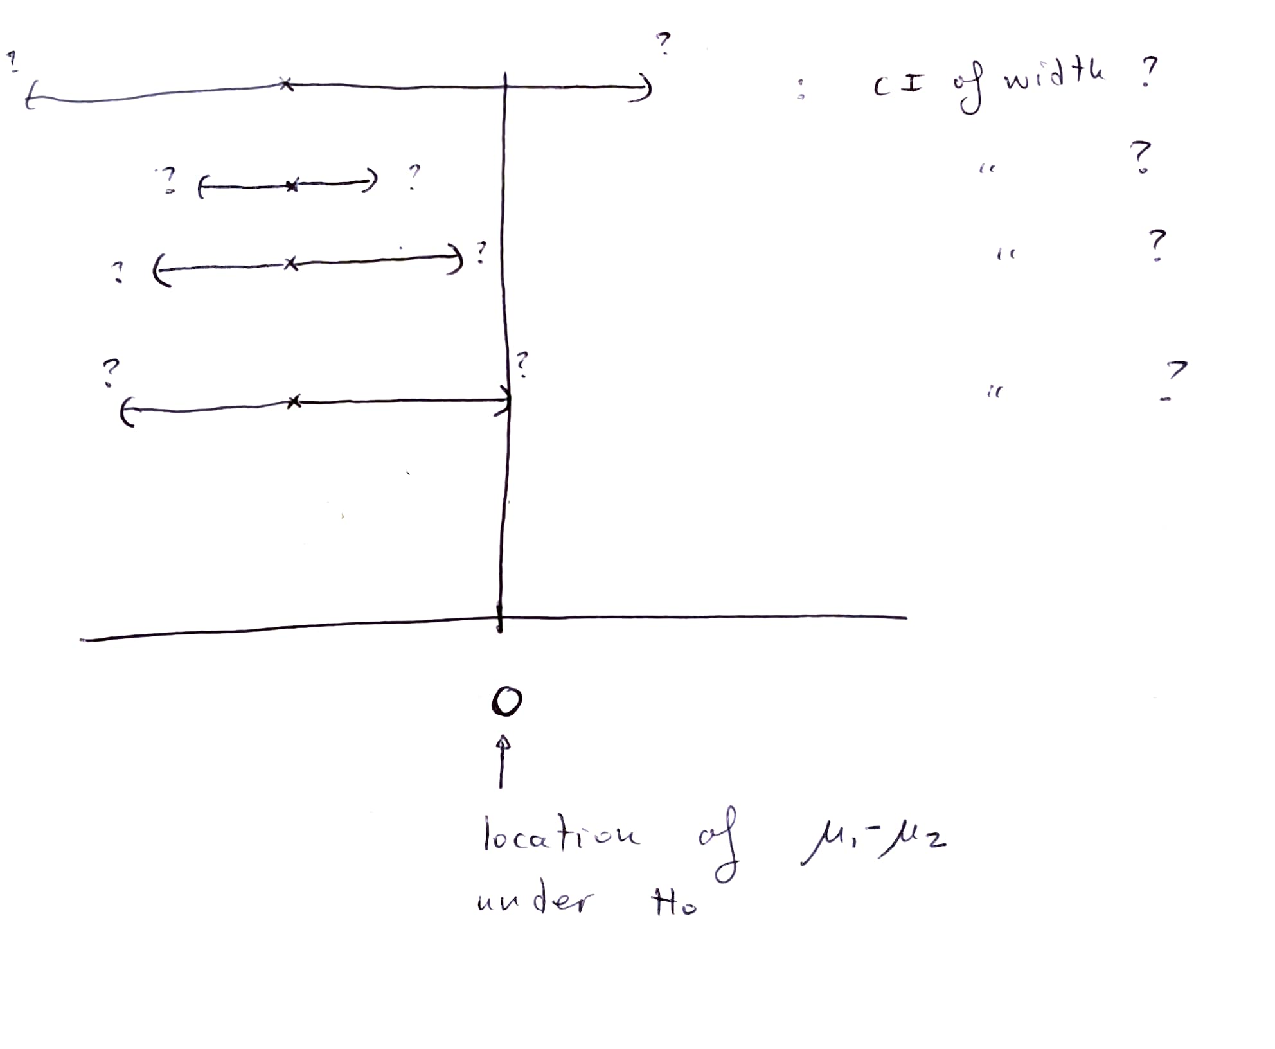
\includegraphics[width=0.80\paperwidth,keepaspectratio]{cittest.pdf}
 \caption{\label{cittest} Fill up the question marks. (Figure not necessarily at scale, but overlaps or not with the 0 line are correct).}
 \end{center}
 \end{figure}

As it says: fill up the question marks.


\end{document}







% <<sewidth,echo=FALSE,results='hide',message=FALSE>>=
% mdiff <- -diff(tt1$estimate)

% ci95 <- t.test(p53 ~ cond, data = dp53, conf.level = 0.95)$conf.int
% ci999 <- t.test(p53 ~ cond, data = dp53, conf.level = 0.999)$conf.int
% ci97 <- t.test(p53 ~ cond, data = dp53, conf.level = 1 - tt1$p.value)$conf.int

% s97 <- (ci97[1] - mdiff)/tt1$statistic
% s95 <- (ci95[1] - mdiff)/q05
% s999 <- (ci999[1] - mdiff)/q001
% @


% And you can check that the width of the confidence intervals is (minor differences are expected from rounding errors et al):

  % <<>>=

% ## 95%
% 2.11 * 0.3838

% ## 97% (i.e., 1 - p.value)
% 2.34 * 0.3838

% ## 999%
% 3.95 * 0.3838
% @
